\chapter{Les R\^oles et Les Utilisateurs}\label{chap:utilisateurs}
\index{types de \roles}

\utilisateurs: \lienadmin, \liencaissier, \liengestionnairedesstocks,
		       \lienmagasinier, \lienmanager, \lienvendeur.\\

\chapintro{Ce chapitre d\'ecrit les diff\'erents types d'utilisateurs de
\yeren: \admin, \caissier, \magasinier, \manager, et \vendeur.}

\nxsection{Introduction}\label{sec:utilisateurs-introduction}

\yeren maintient les donn\'ees suivantes pour chaque utilisateur:
\begin{enumerate}[1)]
	\item l'\'email 
	\item la bo\^ite postale
	\item le date de naissance 
	\item le lieu de naissance 
	\item la localisation (le site de l'entreprise o\`u l'employ\'e
	      est en fonction). Cette valeur ne peut \^etre \'edit\'ee.
	\item le mot de passe \obligatoire
	\item les noms \obligatoire
	\item le nom d'utilisateur \obligatoire
	\item le num\'ero de t\'el\'ephone 1 
	\item le num\'ero de t\'el\'ephone 2 
	\item le pays 
	\item les pr\'enoms \obligatoire
	\item la province ou l\'etat
	\item le r\^ole dans \yeren (\admin, \caissier, \magasinier, \manager, ou \vendeur) \obligatoire
	\item le titre (Dr., Me., Mlle, Mme, Mr, Pr., Prof.) \obligatoire
	\item la ville 
\end{enumerate}

\newpage

\nxsection{Le R\^ole ''Administrateur''}\label{sec:utilisateurs-ladministrateur}
\index{administrateur}
\index{LAdministrateur}

La figure~\ref{fig:fenetre-principale-admin} illustre la
fen\^etre d'acceuil d'un utilisateur avec le \role \admin,
apr\`es qu'il se soit enregistr\'e dans \yeren.\\

\begin{figure}[!htbp]
\centering
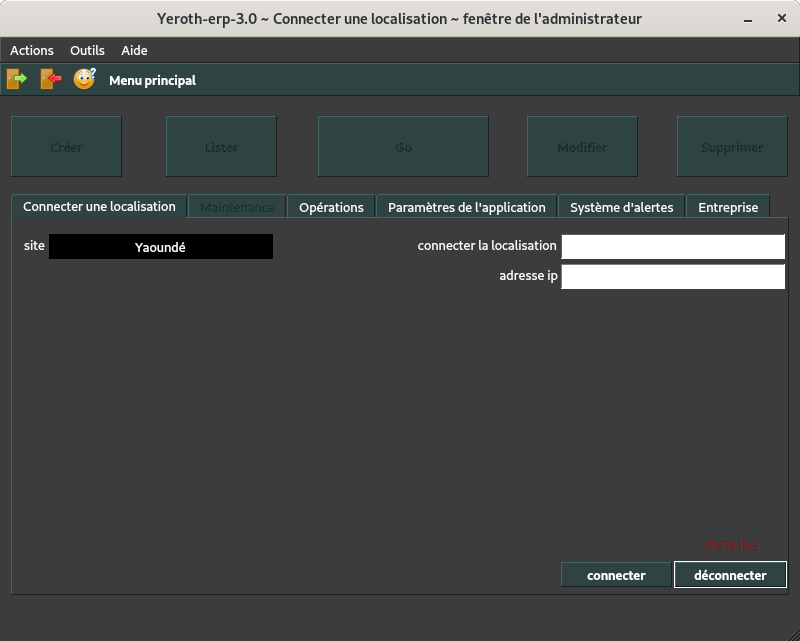
\includegraphics[scale=0.63]{images/yeroth-fenetre-administrateur.png}
\caption{La fen\^etre d'acceuil d'un \admin.}
\label{fig:fenetre-principale-admin}
\end{figure}

Un utilisateur avec le \role \admin a acc\`es aux
fonctionnalit\'es suivantes:
\begin{enumerate}[1)]
	\item arr\^eter le syst\`eme d'alerte
	\item connecter \yerenpos \`a une autre localisation
	\item d\'emarrer le syst\`eme d'alerte
	\item modifier les param\`etres de l'application
	\item modifier les param\`etres du syst\`eme d'alerte.\\   
\end{enumerate}

Un utilisateur avec le \role \admin assume les
t\^aches de cr\'eer et de maintenir les objets suivants:
\begin{enumerate}[1)]
	\item les alertes (sur une p\'eriode de temps, ou sur une quantit\'e en stock)
	%\item les bons de commande
	\item les cat\'egories d'articles
	\item les clients
	\item les comptes utilisateurs
	\item les fournisseurs				
	\item les localisations (une localisation est un site de
	      l'entreprise o\`u se trouve un ou plusieurs stocks).\\   
\end{enumerate}


\newpage

\nxsection{Le R\^ole ''Manager''}\label{sec:utilisateurs-lepatron}
\index{patron}
\index{Manager}

La figure~\ref{fig:yeren-fenetre-patron} illustre la fen\^etre
d'acceuil d'un utilisateur avec le \role \manager, 
apr\`es qu'il se soit enregistr\'e dans \yeroth.\\

\begin{figure}[!htbp]
\centering
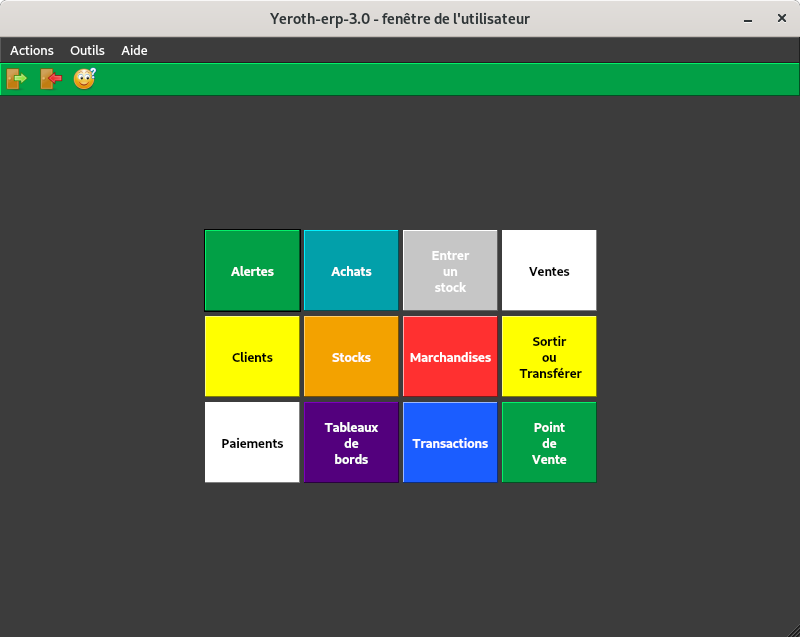
\includegraphics[scale=0.63]{images/yeroth-fenetre-manager.png}
\caption{La fen\^etre d'acceuil d'un \manager}
\label{fig:yeren-fenetre-patron}
\end{figure}

Un utilisateur de \yeroth avec le \role \manager a acc\`es
aux fonctionnalit\'es suivantes:

\begin{enumerate}[1)]
	\item administration (voir chapitre~\ref{chap:administration-logiciel})
	\item gestion des achats (voir chapitre~\ref{chap:gestion-des-achats})
	\item gestion des clients (voir chapitre~\ref{chap:gestion-des-clients})
	\item gestion des stocks (voir chapitre~\ref{chap:gestion-stocks})
	\item gestion des ventes (voir chapitre~\ref{chap:vente})	
	\item mouvements de stocks (voir chapitre~\ref{chap:mouvements-de-stocks})
	\item point de vente (voir chapitre~\ref{chap:vendre})	
	\item syst\`eme d'alertes (voir chapitre~\ref{chap:systeme-dalertes})
	\item tableaux de bords (voir chapitre~\ref{chap:tableaux-de-bords}).\\
\end{enumerate}

\newpage

\nxsection{Le r\^ole ''Manager''}\label{sec:utilisateurs-vendeur}
\index{vendeur}
\index{Vendeur}

La figure~\ref{fig:yeren-fenetre-patron} illustre la fen\^etre
d'acceuil d'un utilisateur avec le \role \manager, 
apr\`es qu'il se soit enregistr\'e dans \yeren.\\

\begin{figure}[!htbp]
\centering
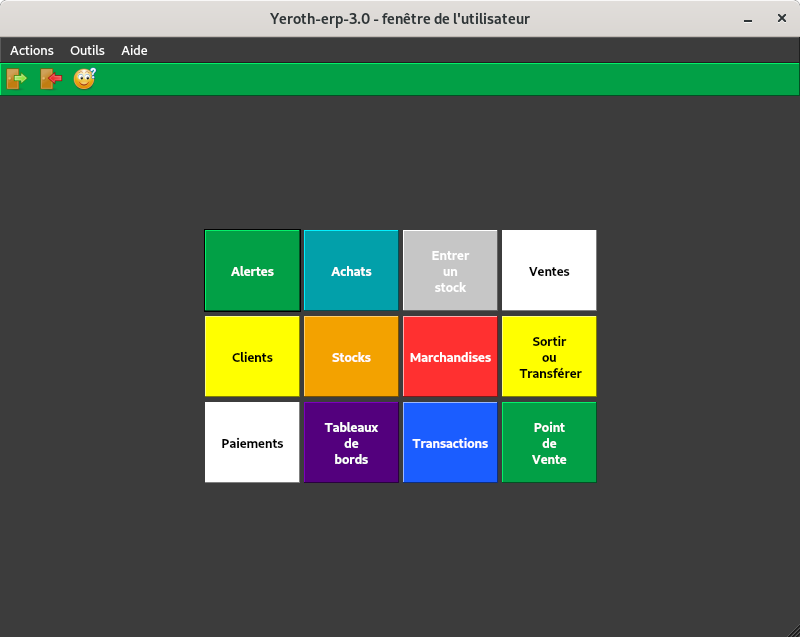
\includegraphics[scale=0.63]{images/yeroth-fenetre-manager.png}
\caption{La fen\^etre d'acceuil d'un ''manager''}
\label{fig:yeren-fenetre-patron}
\end{figure}

Un utilisateur de \yeren avec le \role "\manager" a
acc\`es \`a toutes les fonctionalit\'es de \yeren. Il
cumule les t\^aches de d'administrateur, de magasinier,
et de caissier.

Le \role \manager est le seul \`a donner acc\`es aux
informations des ventes dans leurs totalit\'es, ainsi
qu'\`a la g\'en\'eration et \`a la consultation des
rapports commerciaux.

Le \role \manager est le seul \`a pouvoir consulter toutes
les alertes re\c{c}ues par les autres utilisateurs, et
\`a pouvoir les supprimer.

\newpage

\nxsection{Le R\^ole ''GestionaireDeStocks''}\label{sec:utilisateurs-gestionairedestocks}
\index{gestionaire de stocks}
\index{GestionaireDeStocks}

La figure~\ref{fig:yeren-fenetre-gestionairedestocks} illustre
la fen\^etre d'acceuil d'un utilisateur avec le \role \gestionairedestocks, 
apr\`es qu'il se soit enregistr\'e dans \yeren.\\

\begin{figure}[!htbp]
\centering
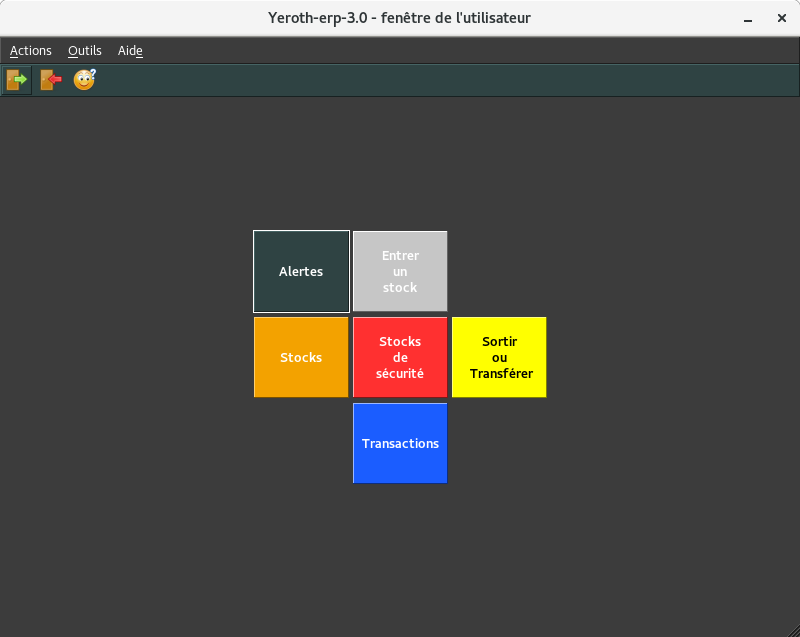
\includegraphics[scale=0.63]{images/yeren-fenetre-gestionairedestocks.png}
\caption{La fen\^etre d'acceuil d'un \gestionairedestocks}
\label{fig:yeren-fenetre-gestionairedestocks}
\end{figure}

Un utilisateur de \yeren avec le \role \gestionairedestocks a acc\`es
aux fonctionnalit\'es suivantes:
\begin{enumerate}[1)]
	\item alertes
	\item gestion des achats
	\item gestion des stocks (voir le Tableau~\ref{tab:taches-fonctions}).\\
\end{enumerate}

\newpage

\nxsection{Le R\^ole ''Magasinier''}\label{sec:utilisateurs-lemagasinier}
\index{magasinier}
\index{LeMagasinier}

La figure~\ref{fig:yeren-fenetre-magasinier} illustre
la fen\^etre d'acceuil d'un utilisateur avec le
\role \magasinier, apr\`es qu'il se soit enregistr\'e
dans \yeren.\\

\begin{figure}[!htbp]
\centering
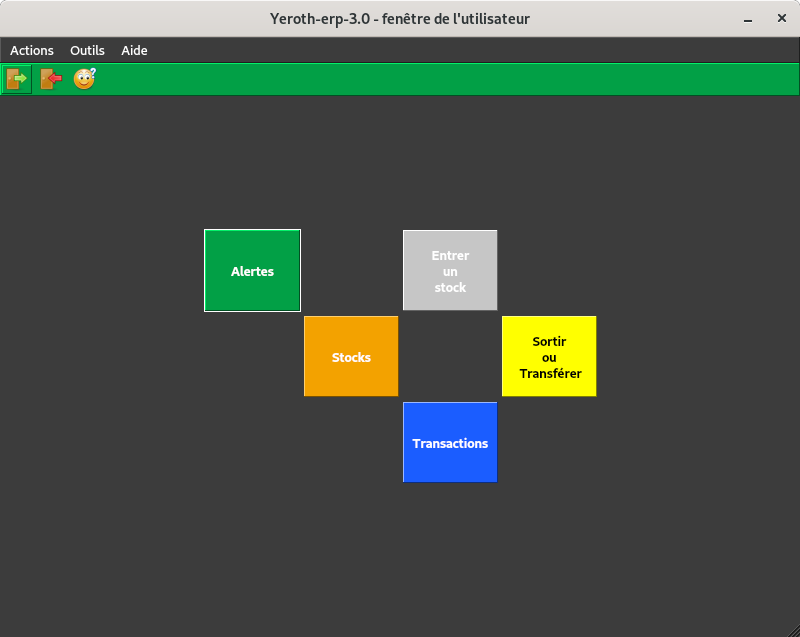
\includegraphics[scale=0.63]{images/yeren-fenetre-magasinier.png}
\caption{La fen\^etre d'acceuil d'un \magasinier.}
\label{fig:yeren-fenetre-magasinier}
\end{figure}

Un utilisateur de \yeren avec le \role \magasinier a acc\`es
aux fonctionnalit\'es suivantes:
\begin{enumerate}[1)]
	\item alertes
	\item gestion des stocks (voir le Tableau~\ref{tab:taches-fonctions}).\\
\end{enumerate}

	
\newpage

\nxsection{Le R\^ole ''Caissier''}\label{sec:utilisateurs-lecaissier}
\index{caissier}
\index{LeCaissier}

La figure~\ref{fig:fenetre-principale-caissier} illustre la
fen\^etre d'acceuil d'un utilisateur avec le \role \caissier,
apr\`es qu'il se soit enregistr\'e dans \yeroth.\\

\begin{figure}[!htbp]
\centering
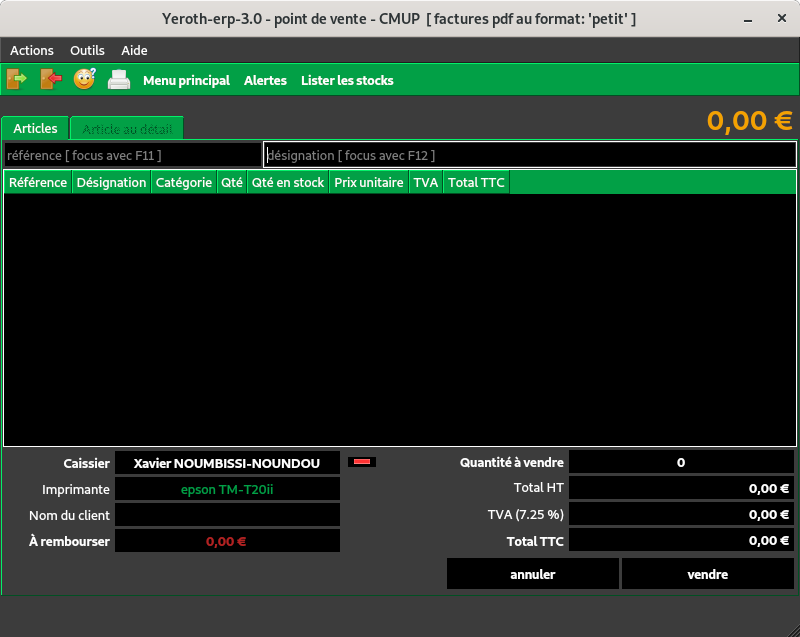
\includegraphics[scale=0.63]{images/yeren-fenetre-caissier.png}
\caption{La fen\^etre d'acceuil d'un \caissier.}
\label{fig:fenetre-principale-caissier}
\end{figure}

Un utilisateur de \yeroth avec le \role \caissier a acc\`es
aux fonctionnalit\'es suivantes:

\begin{enumerate}[1)]
	\item point de vente (voir chapitre~\ref{chap:vendre})
	\item syst\`eme d'alertes (voir chapitre~\ref{chap:systeme-dalertes}).\\
\end{enumerate}
